% !TEX TS-program = pdflatexmk
\documentclass[12pt]{article}

% Layout.
\usepackage[top=1in, bottom=0.75in, left=1in, right=1in, headheight=1in, headsep=6pt]{geometry}

% Fonts.
\usepackage{mathptmx}
\usepackage[scaled=0.86]{helvet}
\renewcommand{\emph}[1]{\textsf{\textbf{#1}}}
\newcommand{\ans}[1][1in]{\rule{#1}{.5pt}}

\usepackage[parfill]{parskip}
\usepackage{adjustbox}

% Misc packages.
\usepackage{amsmath,amssymb,latexsym}
\usepackage{graphicx,hyperref}
\usepackage{array}
\usepackage{xcolor}
\usepackage{multicol,tikz}
\usepackage{tabularx,colortbl,booktabs,xparse}
\usepackage{enumitem}


\usetikzlibrary{calc,trees,positioning,arrows,fit,shapes,through, backgrounds}
\usetikzlibrary{patterns}

% Rotation: \rot[<angle>][<width>]{<stuff>}
\NewDocumentCommand{\rot}{O{45} O{1em} m}{\makebox[#2][l]{\rotatebox{#1}{#3}}}%

\usepackage{fancyhdr}
\pagestyle{fancy} 
\lhead{\large\sf\textbf{MATH F113X: Sortest Edges/Chepaest Link Algorithm for Hamiltonian cycles}}
%\chead{\large\sf\textbf{lecture notes}}
%\rhead{\large\sf\textbf{Day 1}}

\begin{document}
\fbox{The Sorted Edges / Cheapest Link Algorithm}

\textbf{input:} a graph with distances (weights) on the edges

\textbf{output:} a Hamiltonian circuit (or the algorithm fails)

\textbf{strategy:} Add the next cheapest edge to your circuit unless it closes the circuit too soon or creates a degree 3 vertex. Break ties by choosing the alphabetically smallest edge.


%\textbf{Steps:}
%\begin{enumerate}
%	\item (Initialization Step) Choose the cheapest edge in your graph.
%	\item (Iterative Step) 
%		\begin{enumerate} 
%		\item Select the cheapest edge
%		\item If that edge does not complete a circuit too soon and if it does not create a degree-3 vertex, then add it to the list of edges that will cre
%				\end{enumerate} 
%\end{enumerate}

Note that you may have disconnected edges during the process of running the application.

\hrulefill

For convenience, I have listed the edges of the graph in sorted order for you. Draw in the edges as you add them on the empty graph. 

\makeatletter
\newcommand{\Letter}[1]{\@Alph{#1}}
\makeatother

\begin{adjustbox}{valign=t,minipage={.4\textwidth}}
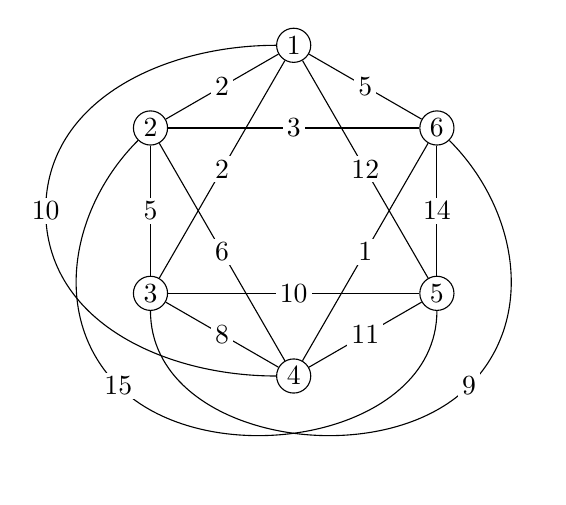
\begin{tikzpicture}[vtx/.style={draw, circle, inner sep =1.5 pt}, lbl/.style =  {inner sep =1.5 pt, fill = white}, scale = .7]
\foreach \i in {0,1,2,3,4,5}{\path let \n1 = {int(\i+1)} in node[vtx] (\i) at (360*\i/6+90:3){\Letter{\n1}};}
\foreach \i in {0,1,2,3,4,5}{
	\draw let \n1 = {int(mod(\i+1, 6))}, \n2 = {int(1*\i+2*\n1)} in (\i) -- node[lbl] {\n2} (\n1);
	\draw let \n3 = {int(mod(\i+2, 6))}, \n4 = {int(mod(3*\i+1*\n3,13)} in (\i) -- node[lbl] {\n4} (\n3);}
\draw (0) to [out=180,in=90] (180:4.5) to [out=270, in=180] (3);
\draw (1) to [out=225,in=135] (225:4.5) to [out=315, in=270] (4);
\draw (2) to [out=270,in=225] (315:4.5) to [out=45, in=315] (5);
\node[inner sep =1.5 pt, fill = white] at (180:4.5){$10$};
\node[inner sep =1.5 pt, fill = white] at (225:4.5){$15$};
\node[inner sep =1.5 pt, fill = white] at (315:4.5){$9$};

\end{tikzpicture}
\end{adjustbox}
\hspace{4cm}
\begin{adjustbox}{valign=t,minipage={.4\textwidth}}
\begin{tikzpicture}[vtx/.style={draw, circle, inner sep =1.5 pt}, lbl/.style =  {inner sep =1.5 pt, fill = white}, scale = .7]
\foreach \i in {0,1,2,3,4,5}{\path let \n1 = {int(\i+1)} in node[vtx] (\i) at (360*\i/6+90:3){\Letter{\n1}};}
%\foreach \i in {0,1,2,3,4,5}{
%	\draw let \n1 = {int(mod(\i+1, 6))}, \n2 = {int(1*\i+2*\n1)} in (\i) -- node[lbl] {\n2} (\n1);
%	\draw let \n3 = {int(mod(\i+2, 6))}, \n4 = {int(mod(3*\i+1*\n3,13)} in (\i) -- node[lbl] {\n4} (\n3);}
%\draw (0) to [out=180,in=90] (180:4.5) to [out=270, in=180] (3);
%\draw (1) to [out=225,in=135] (225:4.5) to [out=315, in=270] (4);
%\draw (2) to [out=270,in=225] (315:4.5) to [out=45, in=315] (5);
%\node[inner sep =1.5 pt, fill = white] at (180:4.5){$10$};
%\node[inner sep =1.5 pt, fill = white] at (225:4.5){$15$};
%\node[inner sep =1.5 pt, fill = white] at (315:4.5){$9$};
%
\end{tikzpicture}
\end{adjustbox}

\begin{adjustbox}{valign=t,minipage={.1\linewidth}}
\begin{tabular}{ c | c | c }
Sorted edges & weight & used? (or why not) \\ \hline
$FD$ & 1 & \\ \hline
$AB$ & 2  &\\ \hline
$AC$ & 2 & \\ \hline
$BF$ & 3 &\\ \hline 
$AF$ & 5& \\ \hline
$BC$ & 5 & \\ \hline
$BD$ & 6& \\ \hline
$CD$ & 8& \\  \hline
$CF$ & 9&\\ \hline
$AD$ & 10&\\ \hline
$CE$ & 10 &\\ \hline
$DE$ & 11&\\ \hline
$AE$ & 12& \\ \hline
$EF$ & 14& \\ \hline
$BE$ & 15&\\ \hline
 \end{tabular}
 \end{adjustbox}

List the vertices of the Hamiltonian circuit, starting at vertex A. 

\hrulefill

What was the weight of the circuit you found? \ans




\newpage

What happens if you apply Sorted Edges/Cheapest Link to the following graph?

\begin{center}
\begin{adjustbox}{valign=t,minipage={.4\textwidth}}
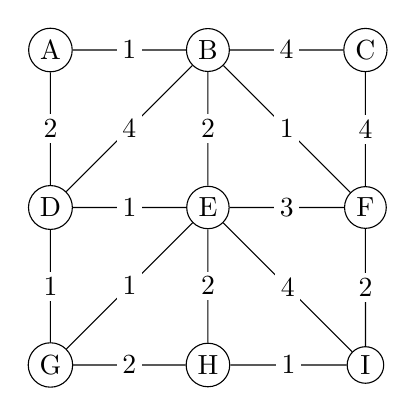
\begin{tikzpicture}[scale = .8]
\tikzstyle{vtx}=[draw, circle, inner sep = 2 pt, node distance=2cm]
\tikzstyle{lbl}=[midway, inner sep = 2 pt, fill = white]

\node[vtx] (A)  {A};
\node[vtx, right of =  A] (B) {B};
\node[vtx, right of = B] (C) {C};
\node[vtx, below of = A] (D) {D};
\node[vtx, below of = B] (E) {E};
\node[vtx, below of = C] (F) {F};
\node[vtx, below of = D] (G) {G};
\node[vtx, below of = E] (H){H};
\node[vtx, below of = F] (I){I};
\draw (A) -- node[lbl]{1} (B) -- node[lbl]{4} (C) -- node[lbl]{4} (F) -- node[lbl]{2} (I) -- node[lbl]{1} (H) -- node[lbl]{2} (G) -- node[lbl]{1} (D)-- node[lbl]{2} (A);
\draw (B) --node[lbl] {2} (E) --node[lbl] {1} (D);
\draw (F) --node[lbl] {3} (E) --node[lbl] {2} (H);
\draw (E) --node[lbl] {1} (G);
\draw (E)--node[lbl] {4} (I);
\draw (B) -- node[lbl] {4} (D);
\draw (B) -- node[lbl] {1} (F);
\end{tikzpicture}
\end{adjustbox}
%%%
%\hfill
%%%%%%%%
\begin{adjustbox}{valign=t,minipage={.4\textwidth}}
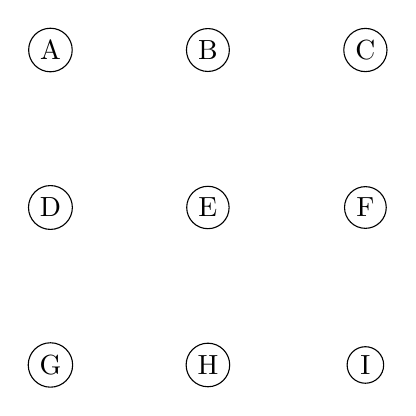
\begin{tikzpicture}
\tikzstyle{vtx}=[draw, circle, inner sep = 2 pt, node distance=2cm]
\tikzstyle{lbl}=[midway, inner sep = 2 pt, fill = white]

\node[vtx] (A)  {A};
\node[vtx, right of =  A] (B) {B};
\node[vtx, right of = B] (C) {C};
\node[vtx, below of = A] (D) {D};
\node[vtx, below of = B] (E) {E};
\node[vtx, below of = C] (F) {F};
\node[vtx, below of = D] (G) {G};
\node[vtx, below of = E] (H){H};
\node[vtx, below of = F] (I){I};
%\draw (A) -- node[lbl]{1} (B) -- node[lbl]{4} (C) -- node[lbl]{3} (F) -- node[lbl]{2} (I) -- node[lbl]{6} (H) -- node[lbl]{5} (G) -- node[lbl]{1} (D)-- node[lbl]{2} (A);
%\draw (B) --node[lbl] {1} (E) --node[lbl] {1} (D);
%\draw (F) --node[lbl] {8} (E) --node[lbl] {2} (H);
%\draw (E) --node[lbl] {1} (G);
%\draw (E)--node[lbl] {4} (I);
\end{tikzpicture}
\end{adjustbox}
%
%\vspace{1cm}
%


\begin{adjustbox}{valign=t,minipage={.5\textwidth}}
\begin{tabular}{ c | c | c }
Sorted edges & weight & used? (or why not) \\ \hline
$AB$ & 1 & \\ \hline
$BF$ & 1  &\\ \hline
$DE$ & 1 & \\ \hline
$DG$ & 1 &\\ \hline 
$EG$ & 1& \\ \hline
$HI$ & 1 & \\ \hline
$AD$ & 2& \\ \hline
 $BE$ & 2& \\  \hline
 \end{tabular}
 \end{adjustbox}
 %
% \hfill
 %
 \begin{adjustbox}{valign=t,minipage={.45\textwidth}}
 \begin{tabular}{ c | c | c }
 %(continued...) & & \\
 Sorted edges & weight & used? (or why not) \\ \hline

$EH$ & 2&\\ \hline
$FI$ & 2&\\ \hline
$GH$ & 2&\\ \hline
$BC$ & 4& \\ \hline
$BD$ & 4& \\ \hline
$CF$ & 4&\\ \hline
$EI$ & 4& \\
\end{tabular}
 \end{adjustbox}
 %%%%%%
 \hfill
 %%%%%%%
%\begin{adjustbox}{valign=t,minipage={.6\linewidth}}
%\begin{tabular}{ c | p{1.5in} | p{1.5in}}
%Used? &edges & weights\\ \hline
%& \\
%& \\
%& \\& \\& \\& \\& \\& \\& \\& \\& \\& \\ & \\& \\
% \end{tabular}
% \end{adjustbox}

\end{center}

%\vspace{1cm}

There is a Hamiltonian circuit on this graph. What is the smallest-weight Hamiltonian circuit you can find? 

Circuit: \ans[3in] Weight: \ans

\begin{adjustbox}{valign=t,minipage={.4\textwidth}}
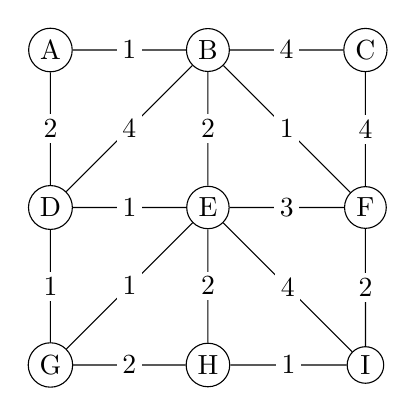
\begin{tikzpicture}[scale = .8]
\tikzstyle{vtx}=[draw, circle, inner sep = 2 pt, node distance=2cm]
\tikzstyle{lbl}=[midway, inner sep = 2 pt, fill = white]

\node[vtx] (A)  {A};
\node[vtx, right of =  A] (B) {B};
\node[vtx, right of = B] (C) {C};
\node[vtx, below of = A] (D) {D};
\node[vtx, below of = B] (E) {E};
\node[vtx, below of = C] (F) {F};
\node[vtx, below of = D] (G) {G};
\node[vtx, below of = E] (H){H};
\node[vtx, below of = F] (I){I};
\draw (A) -- node[lbl]{1} (B) -- node[lbl]{4} (C) -- node[lbl]{4} (F) -- node[lbl]{2} (I) -- node[lbl]{1} (H) -- node[lbl]{2} (G) -- node[lbl]{1} (D)-- node[lbl]{2} (A);
\draw (B) --node[lbl] {2} (E) --node[lbl] {1} (D);
\draw (F) --node[lbl] {3} (E) --node[lbl] {2} (H);
\draw (E) --node[lbl] {1} (G);
\draw (E)--node[lbl] {4} (I);
\draw (B) -- node[lbl] {4} (D);
\draw (B) -- node[lbl] {1} (F);
\end{tikzpicture}
\end{adjustbox}
%%%
\hfill
%%%%%%%%
\begin{adjustbox}{valign=t,minipage={.4\textwidth}}
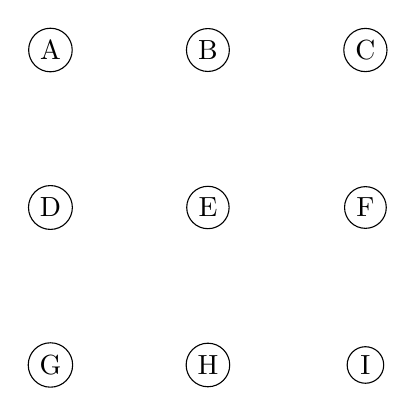
\begin{tikzpicture}[scale = .8]
\tikzstyle{vtx}=[draw, circle, inner sep = 2 pt, node distance=2cm]
\tikzstyle{lbl}=[midway, inner sep = 2 pt, fill = white]

\node[vtx] (A)  {A};
\node[vtx, right of =  A] (B) {B};
\node[vtx, right of = B] (C) {C};
\node[vtx, below of = A] (D) {D};
\node[vtx, below of = B] (E) {E};
\node[vtx, below of = C] (F) {F};
\node[vtx, below of = D] (G) {G};
\node[vtx, below of = E] (H){H};
\node[vtx, below of = F] (I){I};
%\draw (A) -- node[lbl]{1} (B) -- node[lbl]{4} (C) -- node[lbl]{3} (F) -- node[lbl]{2} (I) -- node[lbl]{6} (H) -- node[lbl]{5} (G) -- node[lbl]{1} (D)-- node[lbl]{2} (A);
%\draw (B) --node[lbl] {1} (E) --node[lbl] {1} (D);
%\draw (F) --node[lbl] {8} (E) --node[lbl] {2} (H);
%\draw (E) --node[lbl] {1} (G);
%\draw (E)--node[lbl] {4} (I);
\end{tikzpicture}
\end{adjustbox}

\vspace{1cm}
%
%\begin{adjustbox}{valign=t,minipage={.1\linewidth}}
%\begin{tabular}{ c | c | c }
%Sorted edges & weight & used? (or why not) \\ \hline
%$AB$ & 1 & \\ \hline
%$BF$ & 1  &\\ \hline
%$DE$ & 1 & \\ \hline
%$DG$ & 1 &\\ \hline 
%$EG$ & 1& \\ \hline
%$HI$ & 1 & \\ \hline
%$AD$ & 2& \\ \hline
%$BE$ & 2& \\  \hline
%$EH$ & 2&\\ \hline
%$FI$ & 2&\\ \hline
%$GH$ & 2&\\ \hline
%$BC$ & 4& \\ \hline
%$BD$ & 4& \\ \hline
%$CF$ & 4&\\ \hline
%$EI$ & 4& \\
% \end{tabular}
% \end{adjustbox}
 %%%%%%
 \hfill
 %%%%%%%
%\begin{adjustbox}{valign=t,minipage={.6\linewidth}}
%\begin{tabular}{ c | p{1.5in} | p{1.5in}}
%Used? &edges & weights\\ \hline
%& \\
%& \\
%& \\& \\& \\& \\& \\& \\& \\& \\& \\& \\ & \\& \\
% \end{tabular}
% \end{adjustbox}


%Think of an application of finding a cheapest Hamiltonian cycle that is not the Travelling Salesman Problem.

One strategy for having the algorithm not fail is to turn your graph into a complete graph, and assign very expensive weights (say, 100000) to the ``non-edges''. For example, there is no edge between $G$ and $A$, so you could add edge $AG$ and give it a weight of 10000.

The complete graph on 9 vertices has 36 edges. 
\begin{enumerate}
\item How many edges would you need to add to turn this graph into a complete graph? \ans
\item In this new graph, how many possible Hamiltonian circuits are there? \ans
\end{enumerate}

\end{document}